\documentclass[10pt,a4paper]{article}

\usepackage[utf8x]{inputenc}
\usepackage[norsk]{babel}
\usepackage[T1]{fontenc,url}
\usepackage[hang,small,bf]{caption}
\usepackage{relsize}
\usepackage{setspace}
\usepackage{parskip}
\usepackage{lmodern}
\usepackage{microtype}
\usepackage{verbatim}
\usepackage{amsmath, amssymb, amsthm}
\usepackage{mathtools}
\usepackage{tikz}
\usepackage{physics}
\usepackage{algorithm}
\usepackage{algpseudocode}
\usepackage{listings}
\usepackage{enumerate}
\usepackage{graphicx}
\usepackage{float}
\usepackage{hyperref}
\usepackage{varioref}
\usepackage{siunitx}
\usepackage{todonotes}
\usepackage{color}
\usepackage[margin=3cm]{geometry}
\labelformat{equation}{ligning~(#1)}

\renewcommand{\exp}{\mathrm{e}^}
\newcommand{\halflife}{t_{\frac{1}{2}}}
\newcommand{\half}{\frac{1}{2}}
\newcommand{\planck}{$h = \SI{6.626e-34}{J.s}$}

\definecolor{light_green}{rgb}{0, 0.6, 0}
\definecolor{light_grey}{rgb}{0.5, 0.5, 0.5}
\definecolor{magenta}{rgb}{0.7, 0, 0.5}


\lstdefinestyle{py}{
    language = python,
    frame = single,
    showstringspaces = false,
    basicstyle = \small\ttfamily,
    breaklines = true,
    commentstyle = \color{light_grey},
    keywordstyle = \color{magenta},
    stringstyle = \color{light_green},
}



\begin{document}

\section*{Oppgave E.1 - Koke opp vann}
\addcontentsline{toc}{section}{Oppgave E.1 - Koke opp vann - \texttt{boiling\_water.py}}
Newtons avkjølingslov beskriver hvordan temperaturen $T(t)$ til et objekt forandrer seg over $t$ minutter. 
Den er formulert slik:
\[
\dv{T(t)}{t} = -k\qty(T(t) - T_o) \label{eq:temp}
\]
der $T_o$ er temperaturen til omgivelsen og $k$ er en konstant som forteller hvor mye temperaturen endrer seg per minutt. 

Vi skal se nærmere på hvordan temperaturen til vann ved $15\,\si{\celsius}$ forandrer seg når det kokes opp i en ganske så gammel og slitt vannkoker. Her skal vi bruke Newtons avkjølingslov som en veldig forenkling av hvordan temperaturen vil forandringe seg.
Da er $T(0) = 15\,\si{\celsius}$. Vi setter $k = 0.2$. 

\subsection*{a)}
Vannkokeren får en temperatur lik $100 \si{\celsius}$ med en gang den startes opp. Vi har altså at $T_o= 100\,\si{\celsius}$ for alle $t$ minutter.  

Lag et program som bruker \texttt{ODESolver} for å regne ut temperaturen til vannet $T(t)$. Bruk $N = 1000$ likt fordelte verdier for $t$ som er mellom 0 og 15. 
\subsection*{b)}
Som du kanskje så i a), så tar det ganske lang tid før vannet når $100\si{\celsius}$. En venn av deg prøver å ordne vannkokeren, men uheldigvis greier å gjøre den dårligere. Du gjør noen målinger for å se hvor ille vannkokeren din har blitt, og merker at temperaturen på vannkokeren endrer seg nå slik:
\[
T_o(t) = 20\sin\qty(\frac{\pi}{3}t)+80  \label{eq:ttemp}
\]

Utvid programmet ditt fra a) slik at den løser \vref{eq:temp} med den nye modellen for hvordan temperaturen i vannkokeren er, \vref{eq:ttemp}. 

La programmet ditt plotte temperaturen til vannet $T(t)$ fra a) sammen temperaturen $T(t)$ programmet ditt får i denne deloppgaven. 

Filnavn: \texttt{boiling\_water.py}
\section*{Oppgave E.2 - RC krets}
\addcontentsline{toc}{section}{Oppgave E.2 - RC krets - \texttt{RC.py}}
Hensikten med denne oppgaven er å studere endringen i elektrisk ladning $Q$ holdt av en kondensator over tid.
	
Figur \ref{fig:E2_RC} viser en RC-krets, med en kondensator, en motstand og et batteri. Vi skal konsentrere oss om kondensatoren, som består av to parallelle metalplater. Når vi kobler opp batteriet, vil disse platene lades opp. Når vi kobler fra batteriet, vil kondensatoren utlades ved at strøm går tilbake gjennom kretsen, helt til $Q = \SI{0}{C}$.
	
\begin{center}
	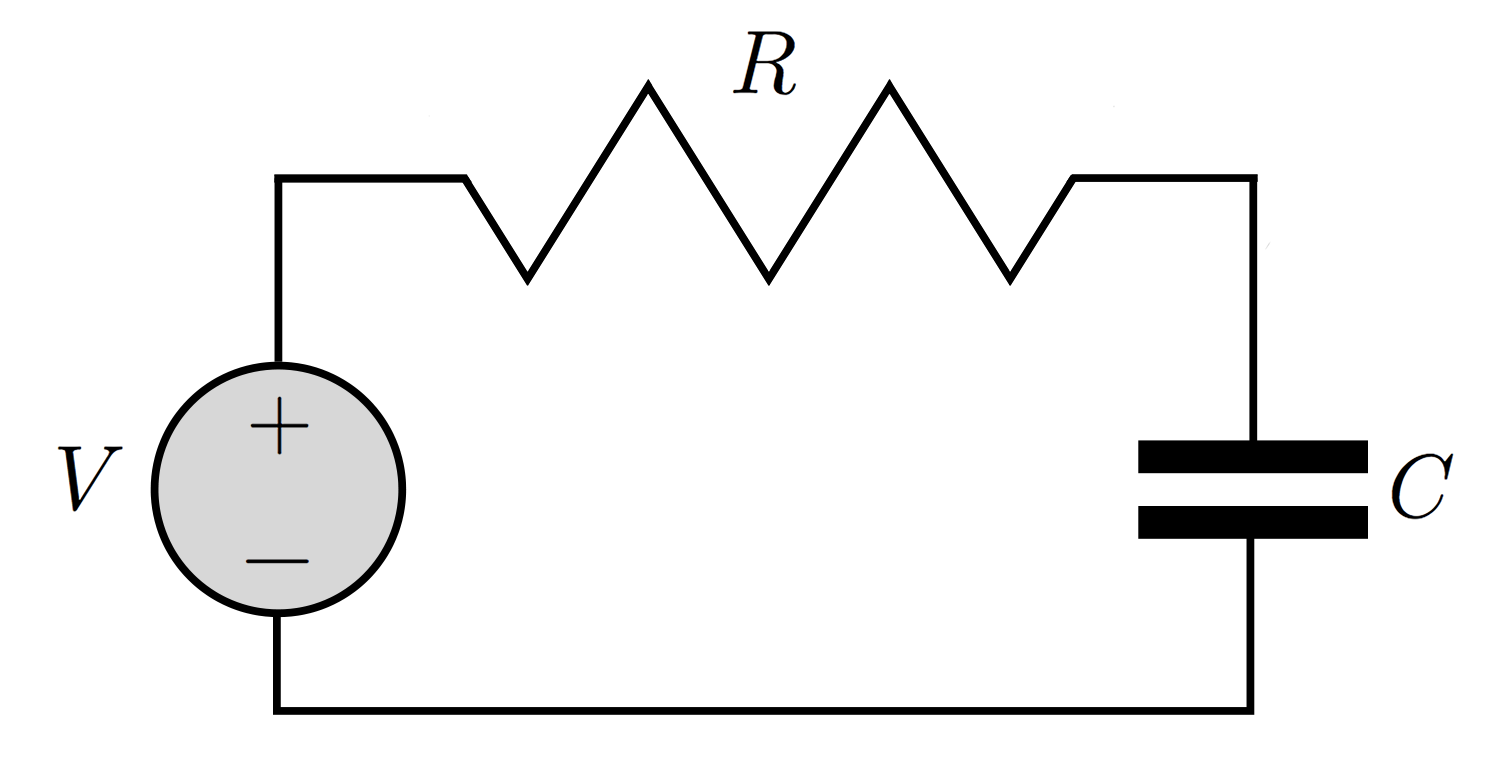
\includegraphics[scale=1]{fig_RC-cp1.png}
	\captionof{figure}{Illustrasjon av en RC-krets.}
    \label{fig:E2_RC}
\end{center}

	
Batteriet har en konstant spenning $V$ (målt i Volt) mens det er på. Motstanden har en resistans $R$ (målt i Ohm) som sier oss hvor godt den hindrer strøm. Kondensatoren har en kapasitans $C$ (målt i Farad).

Ladningen $Q$ holdt av kondensatoren på et tidspunkt $t$ er gitt av differensialligningen
\begin{align}\label{eqn:Qder}
Q'(t) = \frac{V}{R} - Q(t)\frac{1}{RC}
\end{align}

\subsection*{a)}
Bruk \texttt{ODESolver} til å løse for $Q(t)$ over de første 10 sekundende, med 101 tidssteg. Sett batteriets spenning til $V = \SI{8}{Volt}$, kondensatorens kapasitans til $C = \SI{2e-8}{Farad}$, og motstandens resistans til $R = \SI{e8}{Ohm}$. Kapastitatoren har ingen ladning, $Q_0=0$, ved $t=0$. Bruk både Forward Euler og Runge Kutta 4, og plott resultatene fra begge løsningene sammen med den analytiske løsningen
\begin{align}
Q(t) = (Q_0 - CV)\exp{-t/RC} + CV
\end{align}

Studer hvor mye du må redusere antallet tidssteg for å se forskjellen mellom de numeriske løsningene og den analytiske.
	
\subsection*{b)}
Batteriet blir ustabilt på tidspunktet $t=\SI{10}{s}$, og spenningen begynner å oscillere som en sinuskurve. Ved $t = \SI{20}{s}$ slutter batteriet å virke. Vi kan implementere dette i løsningen vår ved å la spenningen fra batteriet være en funksjon av tid, $V(t)$. Vi ser forsatt på differensialligningen $\ref{eqn:Qder}$, men nå er spenningen gitt som
\begin{equation}
V(t) =
\begin{cases}
8,           &t < 10 \\
4\sin(t)+4,  &10 < t < 20 \\
0,           &t > 20
\end{cases}
\end{equation}

Plott den nye løsningen $Q(t)$ over 30 sekunder med Runge Kutta 4 og 101 tidssteg.

Filnavn: \texttt{RC.py}



\section*{Oppgave E.3 - Ballkast med luftmotstand}
\addcontentsline{toc}{section}{Oppgave E.3 - Ballkast med luftmotstand - \texttt{throw\_air\_resistance.py}}
I denne oppgaven skal vi simulere et ballkast der vi inkluderer luftmostand. 
For å gjøre det, skal vi bruke \texttt{ODESolver.py}.

Vinden beveger seg i samme retning som ballen blir kastet. 

Ligningene vi skal løse for å finne ballens posisjon er:
\begin{align*}
	\dv{x}{t} &= v_x \\
	\dv{v_x}{t} &= -\frac{1}{2m}\rho C \pi R^2 \qty(v_x - w)^2 \\
	\hfill \\
	\dv{y}{t} &= v_y \\
	\dv{v_y}{t} &= -g
\end{align*}
der $C = 0.47$ er et mål på hvor mye motstand ballen gjør på luften, $R$ er  radiusen til ballen, $m$ er ballens masse, $v_x$ er ballens fart langs x-aksen, $w$ er farten til vinden og $g = 9.81\,\si{\meter.\per\square\second}$.

Initialbetingelsene for denne modellen er
\begin{align*} 
	x(0) &= 0 \\
	v_x(0) &= v_0\cos\theta
	\hfill \\
	y(0) &= 0 \\
	v_y(0) &= v_0\sin\theta
\end{align*}
der $\theta$ er kastevinkelen og $v_0$ kastefarten (i \si{\meter.\per\second}). 

\subsection*{a)}
Definér en klasse som holder på informasjon om dette problemet. Klassen skal ha samme struktur som klassen \texttt{Problem} på side 790 i boken (eller side 745 hvis du bruker 4. utgave). \\
Klassen i denne oppgaven skal ha en konstruktør som tar inn initialbetingelsene i form av en liste, radiusen $R$ til ballen, ballens masse $m$ og vindfarten $w$. 

Klassen skal også ha en \texttt{\_\_call\_\_}-funksjon som returnerer listen 
\begin{center}
	\texttt{[vx,$ -\dfrac{1}{2m}\rho C \pi R^2 \qty(v_x - w)^2$,vy,$-g$]}  
\end{center}
der \texttt{vx} og \texttt{vy} er funnet på samme måte som i eksempelet på s. 790 (eller 745) i boken. 


\subsection*{b)} 
Vi skal nå se på hvordan vindfarten $w$ påvirker ballens bane over $T = 0.5$ sekunder. 

Anta vi kaster en ball med radius $R = 0.03275\,\si{\meter}$ og masse $m = 0.057\,\si{\kg}$ med en vinkel $\theta = \frac{\pi}{4}$ og kastefart $ v_0 = 10 \,\si{\meter.\per\second}$. Vi lar også $x(0) = 0$ og $y(0) = 0$.


Vi skal se på vindfartene $w = -10,-5,0,5,\text{ og }10$.
For hver vindfart $w$ skal programmet:
\begin{itemize}
\item[1)] Lage en instanse av klassen definert i a) der verdiene for $R$,$m$, $w$ og listen av initialbetingelsene sendes inn.  Listen av initialbetingelsene \texttt{U0} kan ha følgende form:  

\texttt{U0} = \texttt{[x0,vx0,y0,vy0]} der \texttt{x0} = $x(0)$, \texttt{vx0} = $v_0\cos\qty(\theta)$, \texttt{y0} = $y(0)$ og \texttt{vy0} = $v_0\sin\qty(\theta)$. 

\item[2)] La \texttt{ODESolver} løse for posisjonene. Her kan du velge hvilken metode du vil bruke fra \texttt{ODESolver} for å løse ligningssettet. Pass også på å sende inn mange nok verdier for tiden til \texttt{ODESolver } sin funksjon \texttt{solve} for å presise nok resultater. 

\item[3)] Send de funnede fra posisjonene fra punkt 2) til \texttt{plt.plot(x,y)}. Pass på å hente ut de riktige verdiene fra matrisen som \texttt{ODESolver} sin \texttt{solve} returnerer! 
\end{itemize}
Når programmet er ferdig å ha gått gjennom alle verdiene for $w$, skal programmet kalle på \texttt{plt.show()} for å vise fram ballens bane for ulike $w$. 

\textbf{Viktig:} Når du skal plotte flere grafer i ett plott, er det viktig å kunne skille på dem. For å gjøre det, kan vi bruke en liste av strenger som forteller hver som er unikt ved hver graf. Listen kan så sendes som parameter til \texttt{plt.legend} \textit{før} \texttt{plt.show()} kalles. I vårt tilfelle kan vi gjøre følgende:

\lstinputlisting[style=py]{pseudo_E3.py}

for å kunne vite hva vindfarten var ved hver bane. 

Filnavn: \texttt{throw\_air\_resistance.py}


\section*{Oppgave E.4 - Planetbane}
\addcontentsline{toc}{section}{Oppgave E.4 - Planetbane - \texttt{Orbits.py}}
I denne oppgaven skal vi studere banen til jorden rundt solen ved hjelp av andre ordens ODEs. Fordi jordens bane rundt solen er flat, kan vi modellere dette i to dimensjoner, $x$ og $y$.

Newtons gravitasjonslov forteller oss styrken på gravitasjonskreftene mellom to legemer. Hvis vi dekomponerer dette i $x$ og $y$ retninger, og setter det inn i Newtons andre lov, kan vi løse for akselerasjonen:

\begin{equation}
\frac{d^2x}{dt^2} = -G\frac{M_{sol}x}{x^2+y^2} \quad\quad\quad\quad \frac{d^2y}{dt^2}=-G\frac{M_{sol}x}{x^2+y^2}
\label{eqn:E4}
\end{equation}

Her er $M_{sol}$ massen til solen, $G$ er newtons gravitasjonskonstant, og $x$ og $y$ er avstanden fra jorden til solen i $x$ og $y$ retning.

Vi skal bruke astronomiske enheter istedenfor SI enheter, som betyr at vi
\begin{itemize}
\item regner tid i år (yr) istedenfor sekunder.
\item regner avstander i astronomiske enheter (AU) istedenfor meter\footnote{1 AU er den gjennomsnitlige avstanden mellom jorden og solen.}.
\item regner masser i solmasser (SM) istedenfor kilogram.
\end{itemize}
Dette har effekten at
\begin{itemize}
\item gravitasjonskonstanten blir $G = 4\pi^2\,\mathrm{AU^3yr^{-2}SM^{-1}}$.
\item massen til solen blir $M_{sol} = \SI{1}{SM}$.
\item initialposisjonen til jorden blir $x = \SI{1}{AU}$, $y = \SI{0}{AU}$.
\item initialhastigheten til jorden blir $v_x = \SI{0}{AU/yr}$, $v_y = \SI{2\pi}{AU/yr}$.
\end{itemize}

Bruk \texttt{ODESolver} til å løse \ref{eqn:E4} for jordens bevegelse rundt solen i 10 år, med bruk av initialbetingelsene og parameterene beskrevet over.\\
For hjelp med å løse andre ordens ODEs, se læreboken side 799-801.

Plott $y$ mot $x$ for de 10 årene, og (forhåpentligvis) se en sirkulær bane i avstand $\SI{1}{AU}$.

\textbf{Hint:} Matplotlib holder ikke aksene proporsjonale på plott, som kan få en sirkulær bane til å se epiltisk ut. For å løse dette kan du sette inn linjen \texttt{matplotlib.pyplot.axis('equal')}.

Filnavn: \texttt{Orbits.py}


























 
\end{document}
